\documentclass[12pt]{article}


\author{Fabio J. Matos Nieves}
\date{October 20, 2023}
\title{M.O.S.I.S Host Software\\Progress Report \#2}

\usepackage{graphicx}
\usepackage{pdfpages}
\usepackage[subpreambles=true]{standalone}
\usepackage{import}
\usepackage{graphicx}
\usepackage{float}
\usepackage{minted}
\usepackage{hyperref}
\hypersetup{ colorlinks, citecolor=black,
	filecolor=black,
	linkcolor=black,
	urlcolor=blue,
	pdftitle={M.O.S.I.S Host Software Progress Report 2},
	pdfpagemode=FullScreen,
}

\begin{document}
\begin{titlepage}
  \begin{center}
    \large{University of Puerto Rico\\
    Mayagüez Campus\\
    \vspace{\baselineskip}
    Department of Electrical and Computer Engineering}
  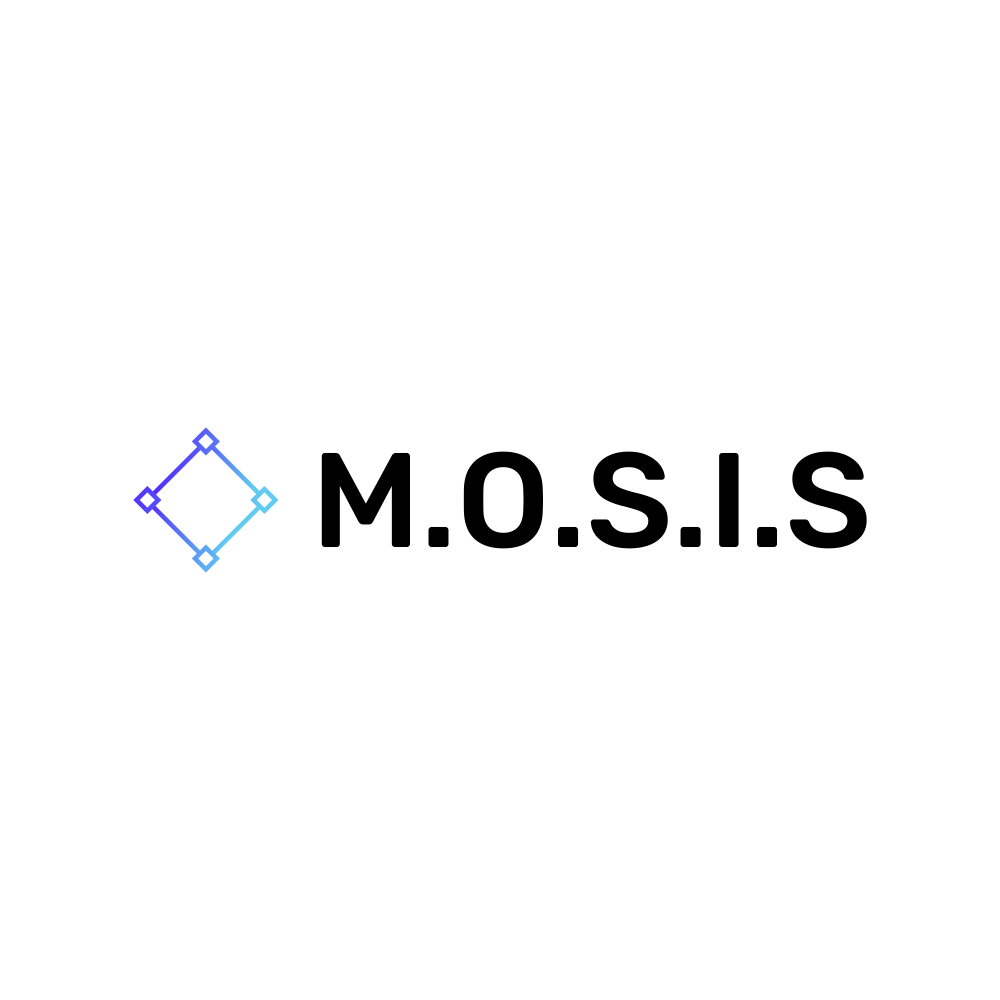
\includegraphics[scale=0.2]{../Title_Page/default.png}\\
    \Huge{\underline{M.O.S.I.S Host Software}\\}
    \Huge{\underline{User Guide}\\}
    \vspace{5cm}
    \large by\\
    Fabio J. Matos Nieves\\
    \normalsize
  \end{center}
\end{titlepage}

\tableofcontents
\newpage
\section{Demonstrations}
\begin{figure}[H]
	\caption{M.O.S.I.S Host Software Front Page}
	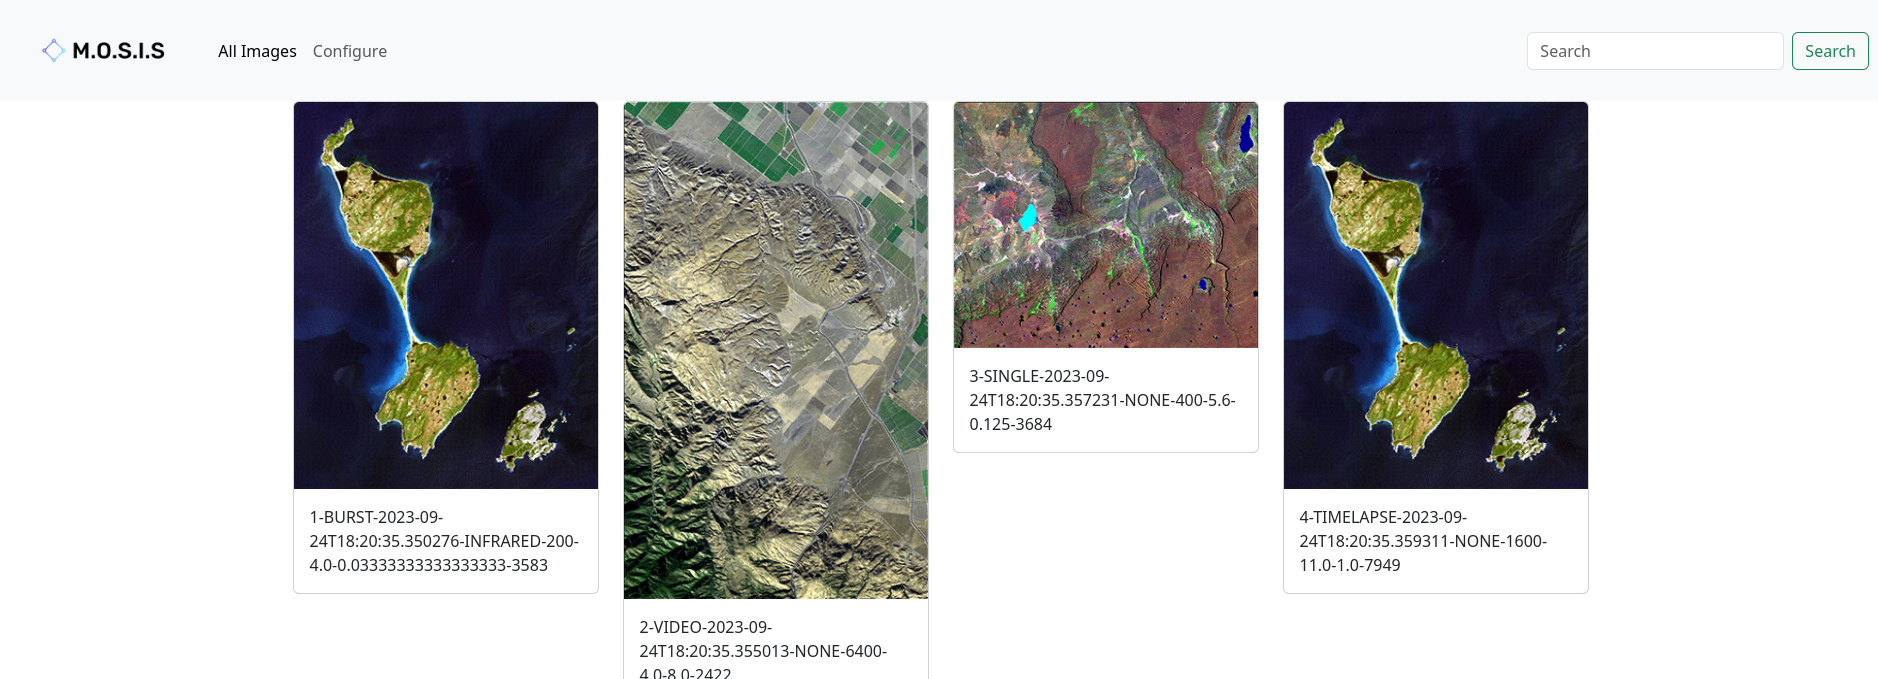
\includegraphics[width=\textwidth]{./Figures/demo_1.png}
\end{figure}
\begin{figure}[H]
	\caption{M.O.S.I.S Host Software Scrolling Front Page}
	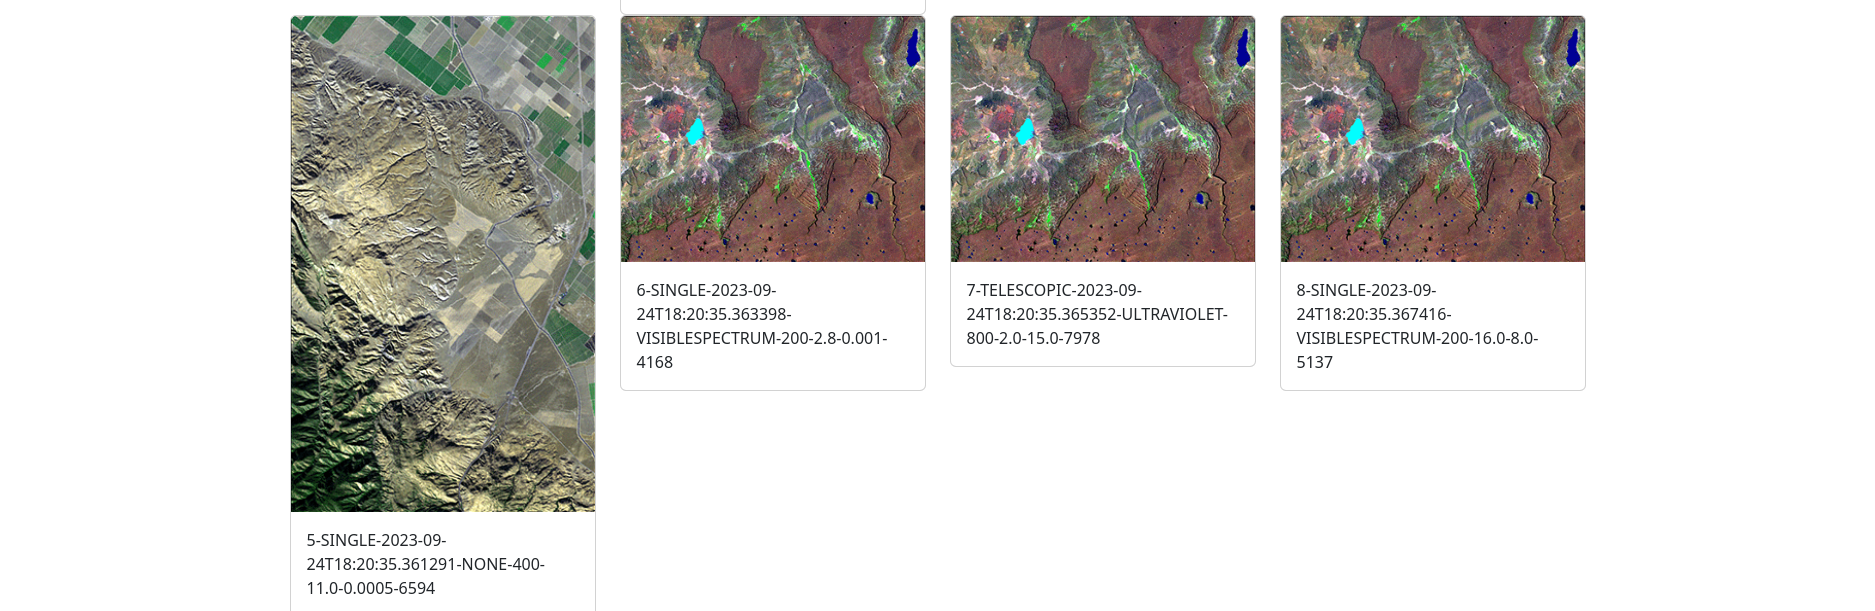
\includegraphics[width=\textwidth]{./Figures/demo_2.png}
\end{figure}
\begin{figure}[H]
	\caption{M.O.S.I.S Host Software Media Entry with Metadata}
	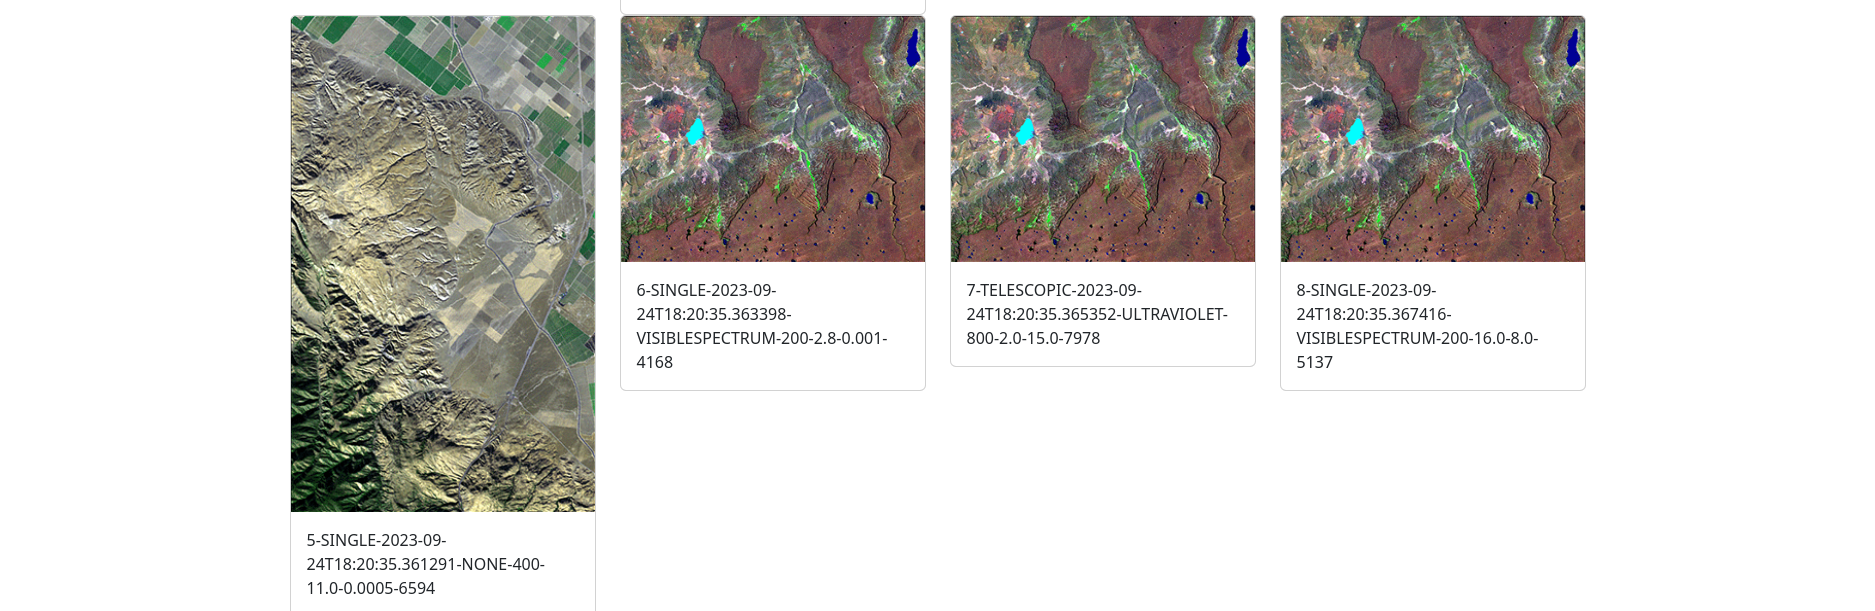
\includegraphics[width=\textwidth]{./Figures/demo_2.png}
\end{figure}
\section{New Features}
\begin{itemize}
	\item Database schema representation in SQLAlchemy
	\item Insertion Statements for MediaEntry and MediaMetadata using SQLAlchemy ORM
	\item Type enforcement when inserting into and reading from database.
	\item Templated front page and media entry pages
	\item Automatic front page generation from database.
	\item Solidified MediaEntry title format
	\item Random: image, pH, temperature, pressure, dissolved oxygen, shot type, illumination type, ISO, aperture size, shutter speed, white balance, MediaEntry and MediaMetaData generators.
	\item Created BASH starup/initialize script for app.py.
\end{itemize}
\section{Usage}
\begin{enumerate}
	\item Download \href{https://www.python.org/downloads/windows/}{Python} and install it.
	\item Download and install \href{https://git-scm.com/download/win}{git}.
	\item Open PowerShell on Windows or a terminal on Mac or Linux.
	\item Type ``python3 --version'' in the terminal and then press enter.
	      \begin{itemize}
		      \item If it does not respond ``Python'' followed by a version number, make sure that the python executable is in the system path.
	      \end{itemize}
	\item Type ``git --version'' in the terminal and press enter.
	      \begin{itemize}
		      \item If it does not respond with ``git version'' followed by a version number, make sure that the git executable is in the system path.
	      \end{itemize}
	\item Clone the M.O.S.I.S repository by typing\\ ``git clone -b research https://github.com/fabiomatos999/M.O.S.I.S.git'' in the terminal and pressing enter. It should start downloading the repository. Wait until you can type again in the terminal.
	\item Change directory to the M.O.S.I.S repository by by typing ``cd M.O.S.I.S'' in the terminal and pressing enter.
	\item Create virtual environment folder by typing ``mkdir venv'' in the terminal and pressing enter.
	\item Create virtual environment by typing ``python -m venv venv'' in the terminal and pressing enter.
	\item Activate virtual environment by executing the Activate.ps1 file inside the scripts directory on Windows or source the activate script based on your shell on Mac or Linux (for more details see \href{https://docs.python.org/3/library/venv.html#how-venvs-work}{here}.)
	\item Install project dependencies by typing\\ ``python3 -m pip install -r requirements.txt'' in the terminal and pressing enter.
	\item Run the host software web server by typing\\ ``python3 -m app'' in the terminal and pressing enter.
	\item Open a web browser
	\item Go to ``127.0.0.1:5000'' in the web browser address box.
	\item The home screen for the M.O.S.I.S host software will open.
\end{enumerate}
\appendix
\section{Technical Specifications}
\begin{itemize}
	\item Python Version 3.11.2
	\item Bootstrap Version: 5.3.2
	\item Flask Version: 3.1.1
	\item SQLAlchemy Version: 2.0.20
	\item Flask-SQLAlchemy Version: 3.1.1
	\item Media Entry Format: entryId-shotType-timeStamp-illuminationType-ISO-apertureSize-shutterSpeed-whiteBalance
\end{itemize}
\section{Host Software Architecture}
\begin{figure}[H]
	\resizebox{\textwidth}{!}{
		\import{./Figures}{class_diagram}
	}
	\caption{M.O.S.I.S Host Software Class Diagram}
\end{figure}
\begin{figure}[H]
	\resizebox{\textwidth}{!}{
		\import{./Figures}{ER_diagram}
	}
	\caption{M.O.S.I.S Host Software Entity Relationship Diagram}
\end{figure}
\section{app.py Documentation}
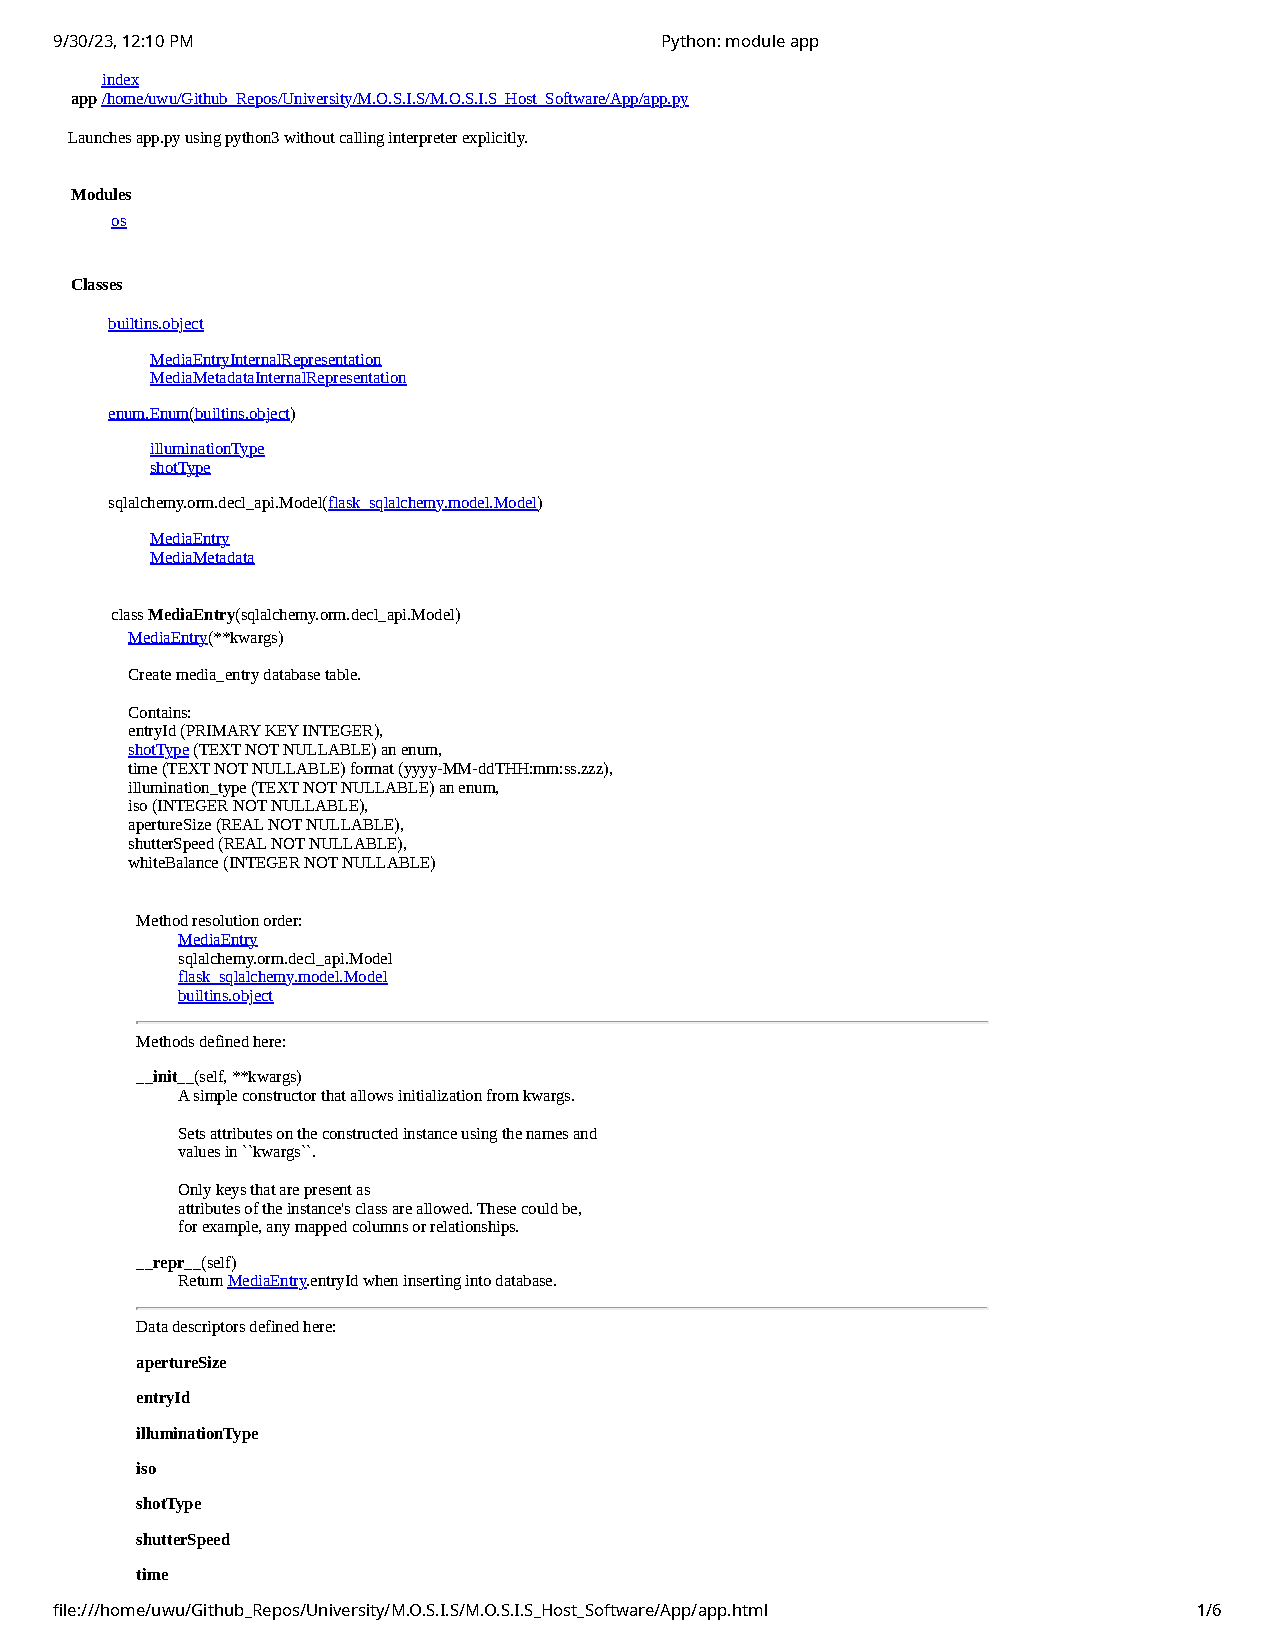
\includepdf[pages=-]{./Figures/app.py_documentation.pdf}
\section{testDataGenerator.py Documenatation}
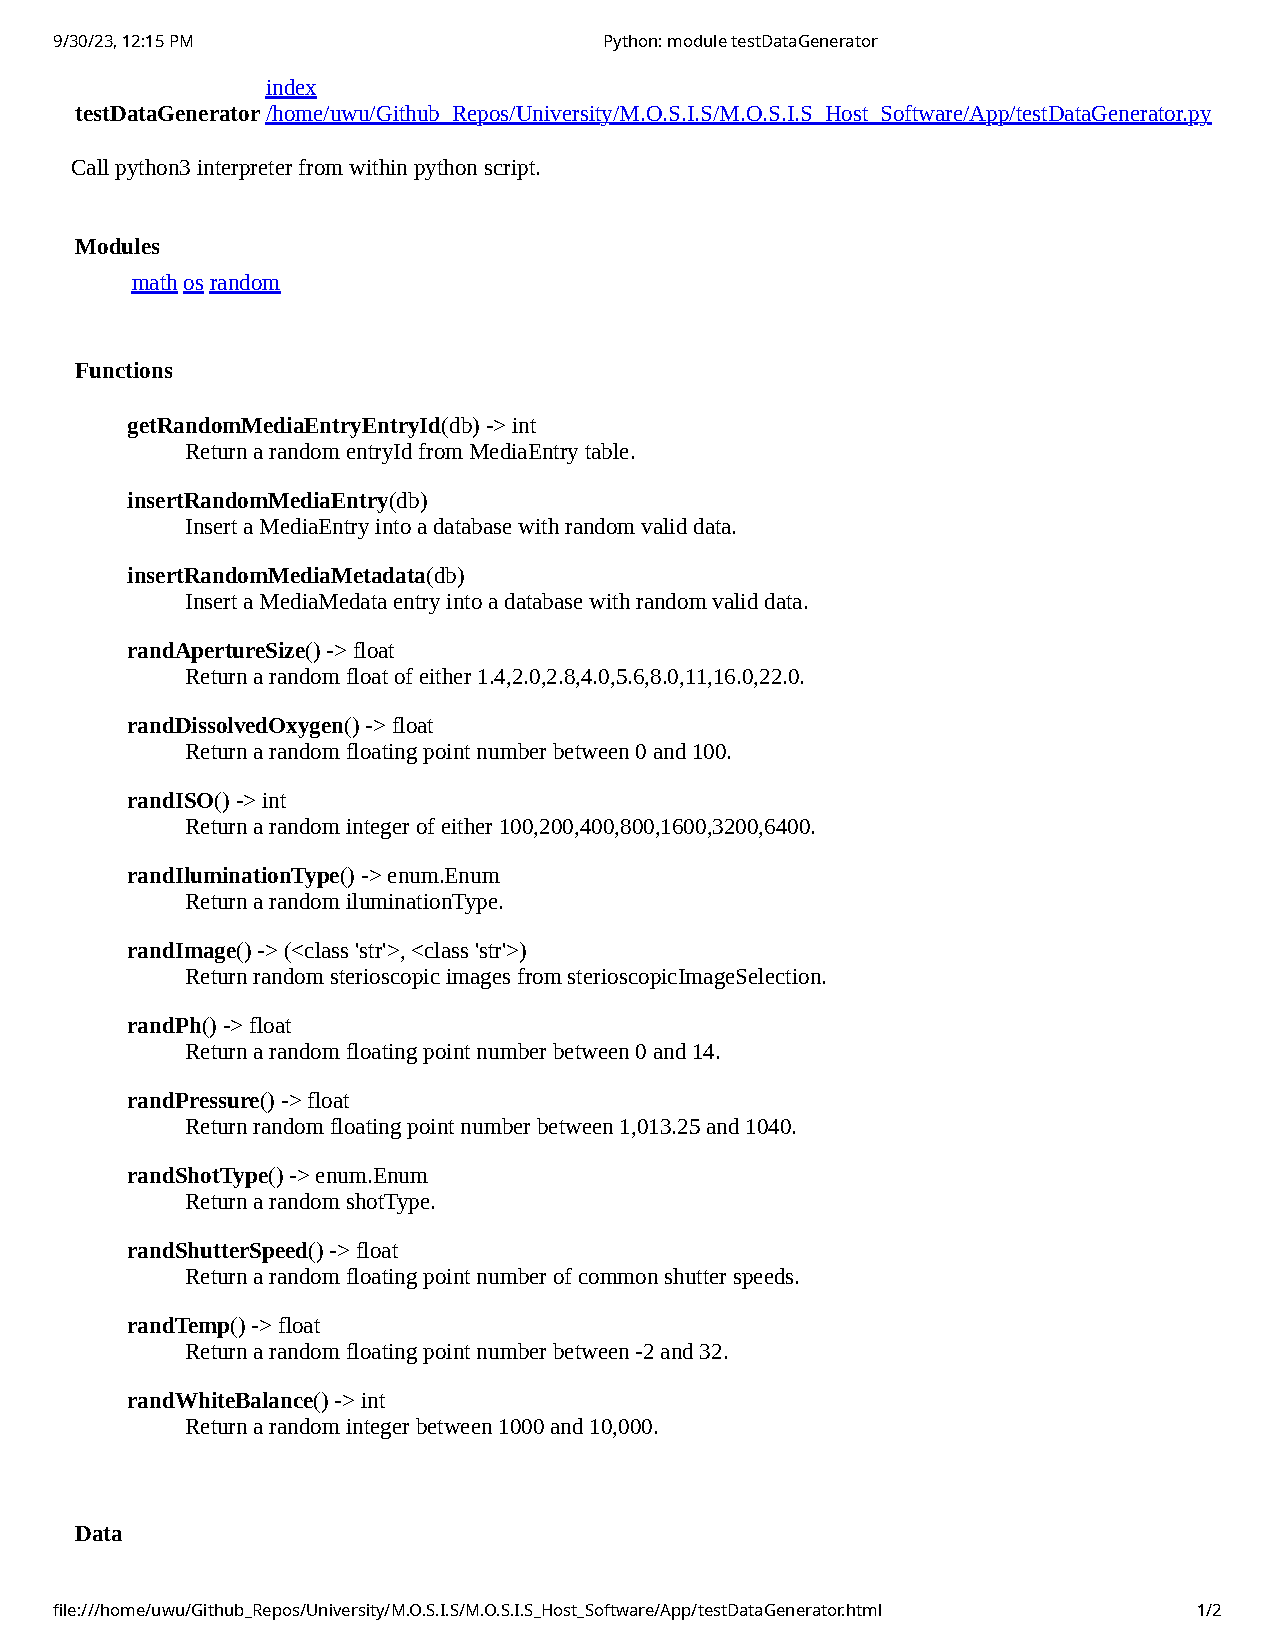
\includepdf[pages=-]{./Figures/testDataGenerator.py_documentation.pdf}
\section{Source Code}
\subsection{app.py}
\inputminted{python}{../../../App/app.py}
\subsection{testDataGenerator}
\inputminted{python}{../../../App/testDataGenerator.py}
\subsection{HTML Templates}
\subsubsection{base.html}
\inputminted[breaklines]{htmldjango}{../../../App/templates/base.html}
\subsubsection{index.html}
\inputminted[breaklines]{htmldjango}{../../../App/templates/index.html}
\subsubsection{entry.html}
\inputminted[breaklines]{htmldjango}{../../../App/templates/entry.html}
\end{document}